\chapter{Introduction}

In many computer science courses, students complete programming assignments to help them learn concepts introduced in class. In these assignments, students often need to read data from an input file, process the data according to the assignment specification, and finally write their results to an output file.

Many of these assignments are evaluated based on correctness through automated testing. To evaluate correctness, the student's output is compared against an instructor provided solution and the number of correct matches determines the student's final mark.

This approach is generally sufficient for introductory programming courses due to the simplicity of the problems. Ideally every student assignment should be reviewed by a human reader, similar to code reviews in the software industry, so that students can develop good coding styles early on in their careers. This also avoids one pitfall of input/output automated testing---ensuring students actually implemented the assignment specifications rather than getting lucky through incorrect or disallowed implementations such as using built-in libraries or generating random outputs.

In recent years at the University of Waterloo, there has been a continual increase in enrollment in programming-related programs (see Figure~\ref{fig:intro-enrollment}). It is not uncommon for early-year courses to have hundreds of enrolled students. For example, the Fall 2018 offering of CS115, an introductory programming course, has over 900 enrolled students \cite{uwaterloo-cs115}.

\begin{figure}
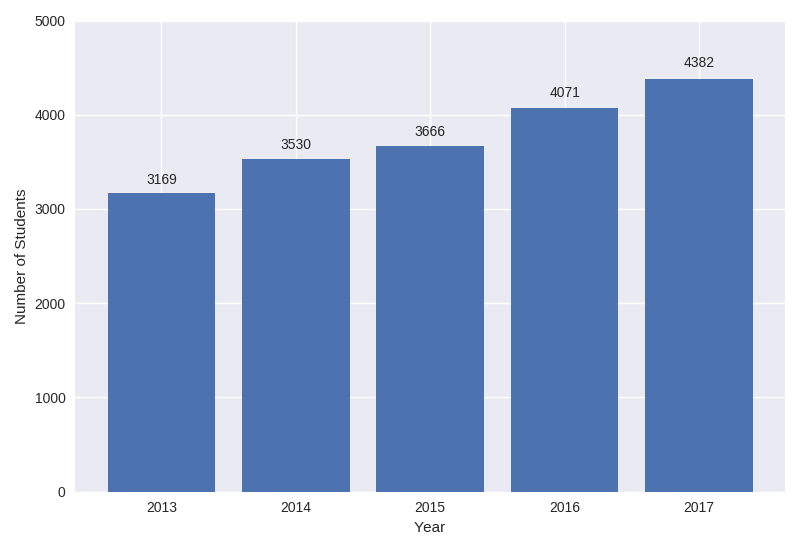
\includegraphics[width=\textwidth]{enrollment}
\caption[Enrollment at University of Waterloo]{The number of students enrolled in the Computer Science, Computer Engineering, or Software Engineering programs at the University of Waterloo continues to rise over the years \cite{uwaterloo-enrollment}.}
\label{fig:intro-enrollment}
\end{figure}

With such large classes, it becomes near-impossible to manually mark every assignment. In the past, hiring more markers was a temporary fix to this growing problem. However, this solution does not scale well because of the increased collaboration needed between markers to ensure consistency in marking. This is especially important for subjective criteria like code style that often has no \textquote{correct} answer. While marker inconsistency may be mitigated by rubrics to some extent, it still requires a deep understanding between markers.

As a result, programming assignments are generally not manually marked until the upper years where class sizes are only a couple dozen students. In rare cases, popular upper-year programming courses such as ECE459, a concurrency programming course, have hundreds of students.

Historically in ECE459, a marker would first compile and run the student's program, aided with an automated script, to eliminate trivial failures such as failed compilations or incorrect output. The marker would then manually inspect the code to check for correct usage of concurrency constructs.

One of the most common complaints amongst past markers for this course was that manually reviewing code is extremely tedious. In addition, manual marking can be error-prone because student code can greatly vary and can be hard to reason through.

%------------------------------------------------------------------------------
\section{Motivating Examples}
\label{sec:intro-motivating-examples}
%------------------------------------------------------------------------------

For the purpose of building a prototype automated marking tool, we focus our efforts on two assignments from ECE459 (see Figure~\ref{fig:intro-nonblockingio} and Figure~\ref{fig:intro-parallelprocessing}) \cite{uwaterloo-ece459}. In these assignments, the students have been provided with a working serial version of a program written in C. The program is a client that calls a web server using the cURL library. The web server, after a random delay, returns a random fragment of an image. The client program then repeats the process until it has received all the fragments. It then stitches them together to reconstruct the original image. Since the web server is on campus, the response time without the delay is usually under 20 ms. We add a Gaussian random delay to simulate network lag and prevent student programs from overwhelming the server. The students are tasked to rewrite the client with non-blocking IO constructs from the cURL library \cite{lib-curl} and again with parallelism constructs from the Pthread library \cite{lib-pthread}. Since the output of all three programs, the reconstructed image, is exactly the same, only manual code inspection can ensure students have actually fulfilled the assignment specifications.

In theory, a correctly parallelized algorithm should execute faster and use more CPU cores than its non-parallel counterpart. One might think that we should be able to check correctness by limiting the run time and checking CPU usage; however, there are a number of problems with this idea.

Firstly, there were always at least a dozen students in every class with poor programming habits who could correctly use the APIs but still have horrible run times. While these students should be penalized, their remark requests and complaints often deter markers from making deductions. To further avoid student complaints, the markers often err on the side of caution and give students a generous timeout limit that even non-parallel algorithms can pass.

Secondly, if malicious students knew that we were checking for CPU usage, they could potentially create fake threads that busy-wait to run alongside the unmodified serial algorithm.

Thirdly, due to the network delay and the possibility of receiving duplicate fragments, a program could potentially take an unpredictably long time before it can reconstruct the final image. 

Therefore, solely relying on automated input/output testing in addition to limiting the runtime or checking CPU usage in this course is insufficient to fully assess students' ability to correctly use the concurrency constructs.

\begin{figure}
\lstinputlisting[language=C, escapechar=]{../media/code/paster_nbio.c}
\caption[Non-Blocking IO Assignment]{The Non-Blocking IO assignment requires rewriting the serial program to use non-blocking  calls in the cURL library. This sample solution shows the key parts of the program that a human marker would look at, such as the cURL library function calls, and their relation to control-flow constructs, such as while-loops and if-statements.}
\label{fig:intro-nonblockingio}
\end{figure}

\begin{figure}
\lstinputlisting[language=C, escapechar=]{../media/code/paster_parallel.c}
\caption[Parallel Processing Assignment]{The Parallel Processing assignment requires the use of parallelism provided by the Pthread library. This assignment is slightly simpler than the Non-Blocking IO assignment because the student simply has to move the key components of the serial program into an isolated function that is then passed to \texttt{pthread\_create}. In this assignment, the marker has to check for the correct usage of \texttt{pthread\_*} functions and ensure proper shared memory protection with mutexes.}
\label{fig:intro-parallelprocessing}
\end{figure}

%------------------------------------------------------------------------------
\section{Approach}
%------------------------------------------------------------------------------

As described in Section~\ref{sec:intro-motivating-examples}, the manual work for markers is straightforward and checklist-like. Our goal is to encode these steps into an automated program to reduce the time needed for marking. It is important to note that we are already automating the compilation and execution of student programs to check for trivial failures (e.g. failed compilations or segmentation faults); our ultimate goal is to further augment this step to also include automated code inspection.

We hypothesize that the ASTs for correct solutions tend to be more similar to each other than incorrect solutions. The intuition behind our idea is that, in the context of programming assignments, there are a limited number of ways to effectively use the concurrency constructs. We assume students will not purposely spend excessive and unnecessary amounts of time to obscure their code or deviate from the standard code examples from class or from online tutorials.

As a result, markers generally look at certain library function calls with relation to the program structure and skim over everything else. For example, to check for correct usage in the Parallel Processing assignment (Figure~\ref{fig:intro-parallelprocessing}), a marker would check to see if \texttt{pthread\_create} and \texttt{pthread\_join} are inside loops but are not in the same loop. They would generally ignore the rest of the boilerplate code such as parameter validation and garbage collection.

From this idea, we built the ClangAutoMarker tool to automate the manual code inspection step of marking. As its name implies, this tool is built on top of the Clang and LLVM infrastructure \cite{lib-llvm}. It first leverages the Clang front-end to parse a student solution and an instructor-provided reference solution into their respective ASTs. It then post-processes these tree data structures and computes the tree edit distance\footnote{A tree $T_1$ can be converted to another tree $T_2$ through a series of steps (i.e. add, remove, or rename nodes in $T_1$ until it is equal to $T_2$). Each step also has an associated cost through a cost function $F$. The tree edit distance is the series of steps that would result in the minimum net cost to convert $T_1$ into $T_2$.} between the student solution's AST and the reference solution's AST. We then repeat this process for all the reference solutions; there are multiple reference solutions because most programming assignments have multiple valid approaches. Finally we normalize and aggregate the edit distances into a single mark between 0 to 100 for the student.

However in practice we would only accept an automated mark if it was a full mark of 100; we require manual review for assignments that did not receive full marks because these automated deductions do not have meaningful feedback relevant for a student, other than the fact that they were notably different from the reference solutions. 

This distinction does not significantly hinder the effectiveness of our tool because, traditionally, the course staff of ECE459 perfers to have a large number of students getting full marks despite having minor or benign problems with their code.
